\section{Visualisations of  K-Means results}
\label{annexe:kmeans_visualizations}

\subsection{Bayesian Optimization and Optimized K-Means ($K=8$)}

\paragraph{Bayesian Optimization Convergence}
The optimization objective remains constant across iterations, indicating that the Bayesian optimization process did not effectively explore the hyperparameter space.

\paragraph{Parameter Space Exploration}
All tested values of $K$ yield nearly identical scores. As a result, the selection of $K=8$ is not statistically supported by the optimization results.

\paragraph{Optimized Clustering Analysis}
The first principal component explains $99.83\%$ of the total variance, indicating that the data is effectively one-dimensional. The presence of vertically aligned clusters in the PCA projection suggests over-segmentation and confirms that $K=8$ exceeds the intrinsic structure of the data.

\paragraph{Clustering Metrics Comparison}
Compared to the default configuration ($K=3$), the Silhouette score decreases (from $0.71$ to $0.60$), indicating reduced cluster separation. Although the Davies--Bouldin index improves and the Calinski--Harabasz index increases, these improvements primarily reflect increased compactness and sensitivity to higher $K$ rather than better structural clustering.

\paragraph{Inertia Analysis}
A significant reduction in inertia is observed for $K=8$. However, since inertia decreases monotonically with the number of clusters, this result alone does not indicate improved clustering quality.

\paragraph{Summary}
While $K=8$ produces more compact clusters according to internal metrics, it leads to over-segmentation and reduced interpretability. The optimized solution is therefore mathematically tighter but structurally less meaningful.

\begin{figure}[H]
    \centering
    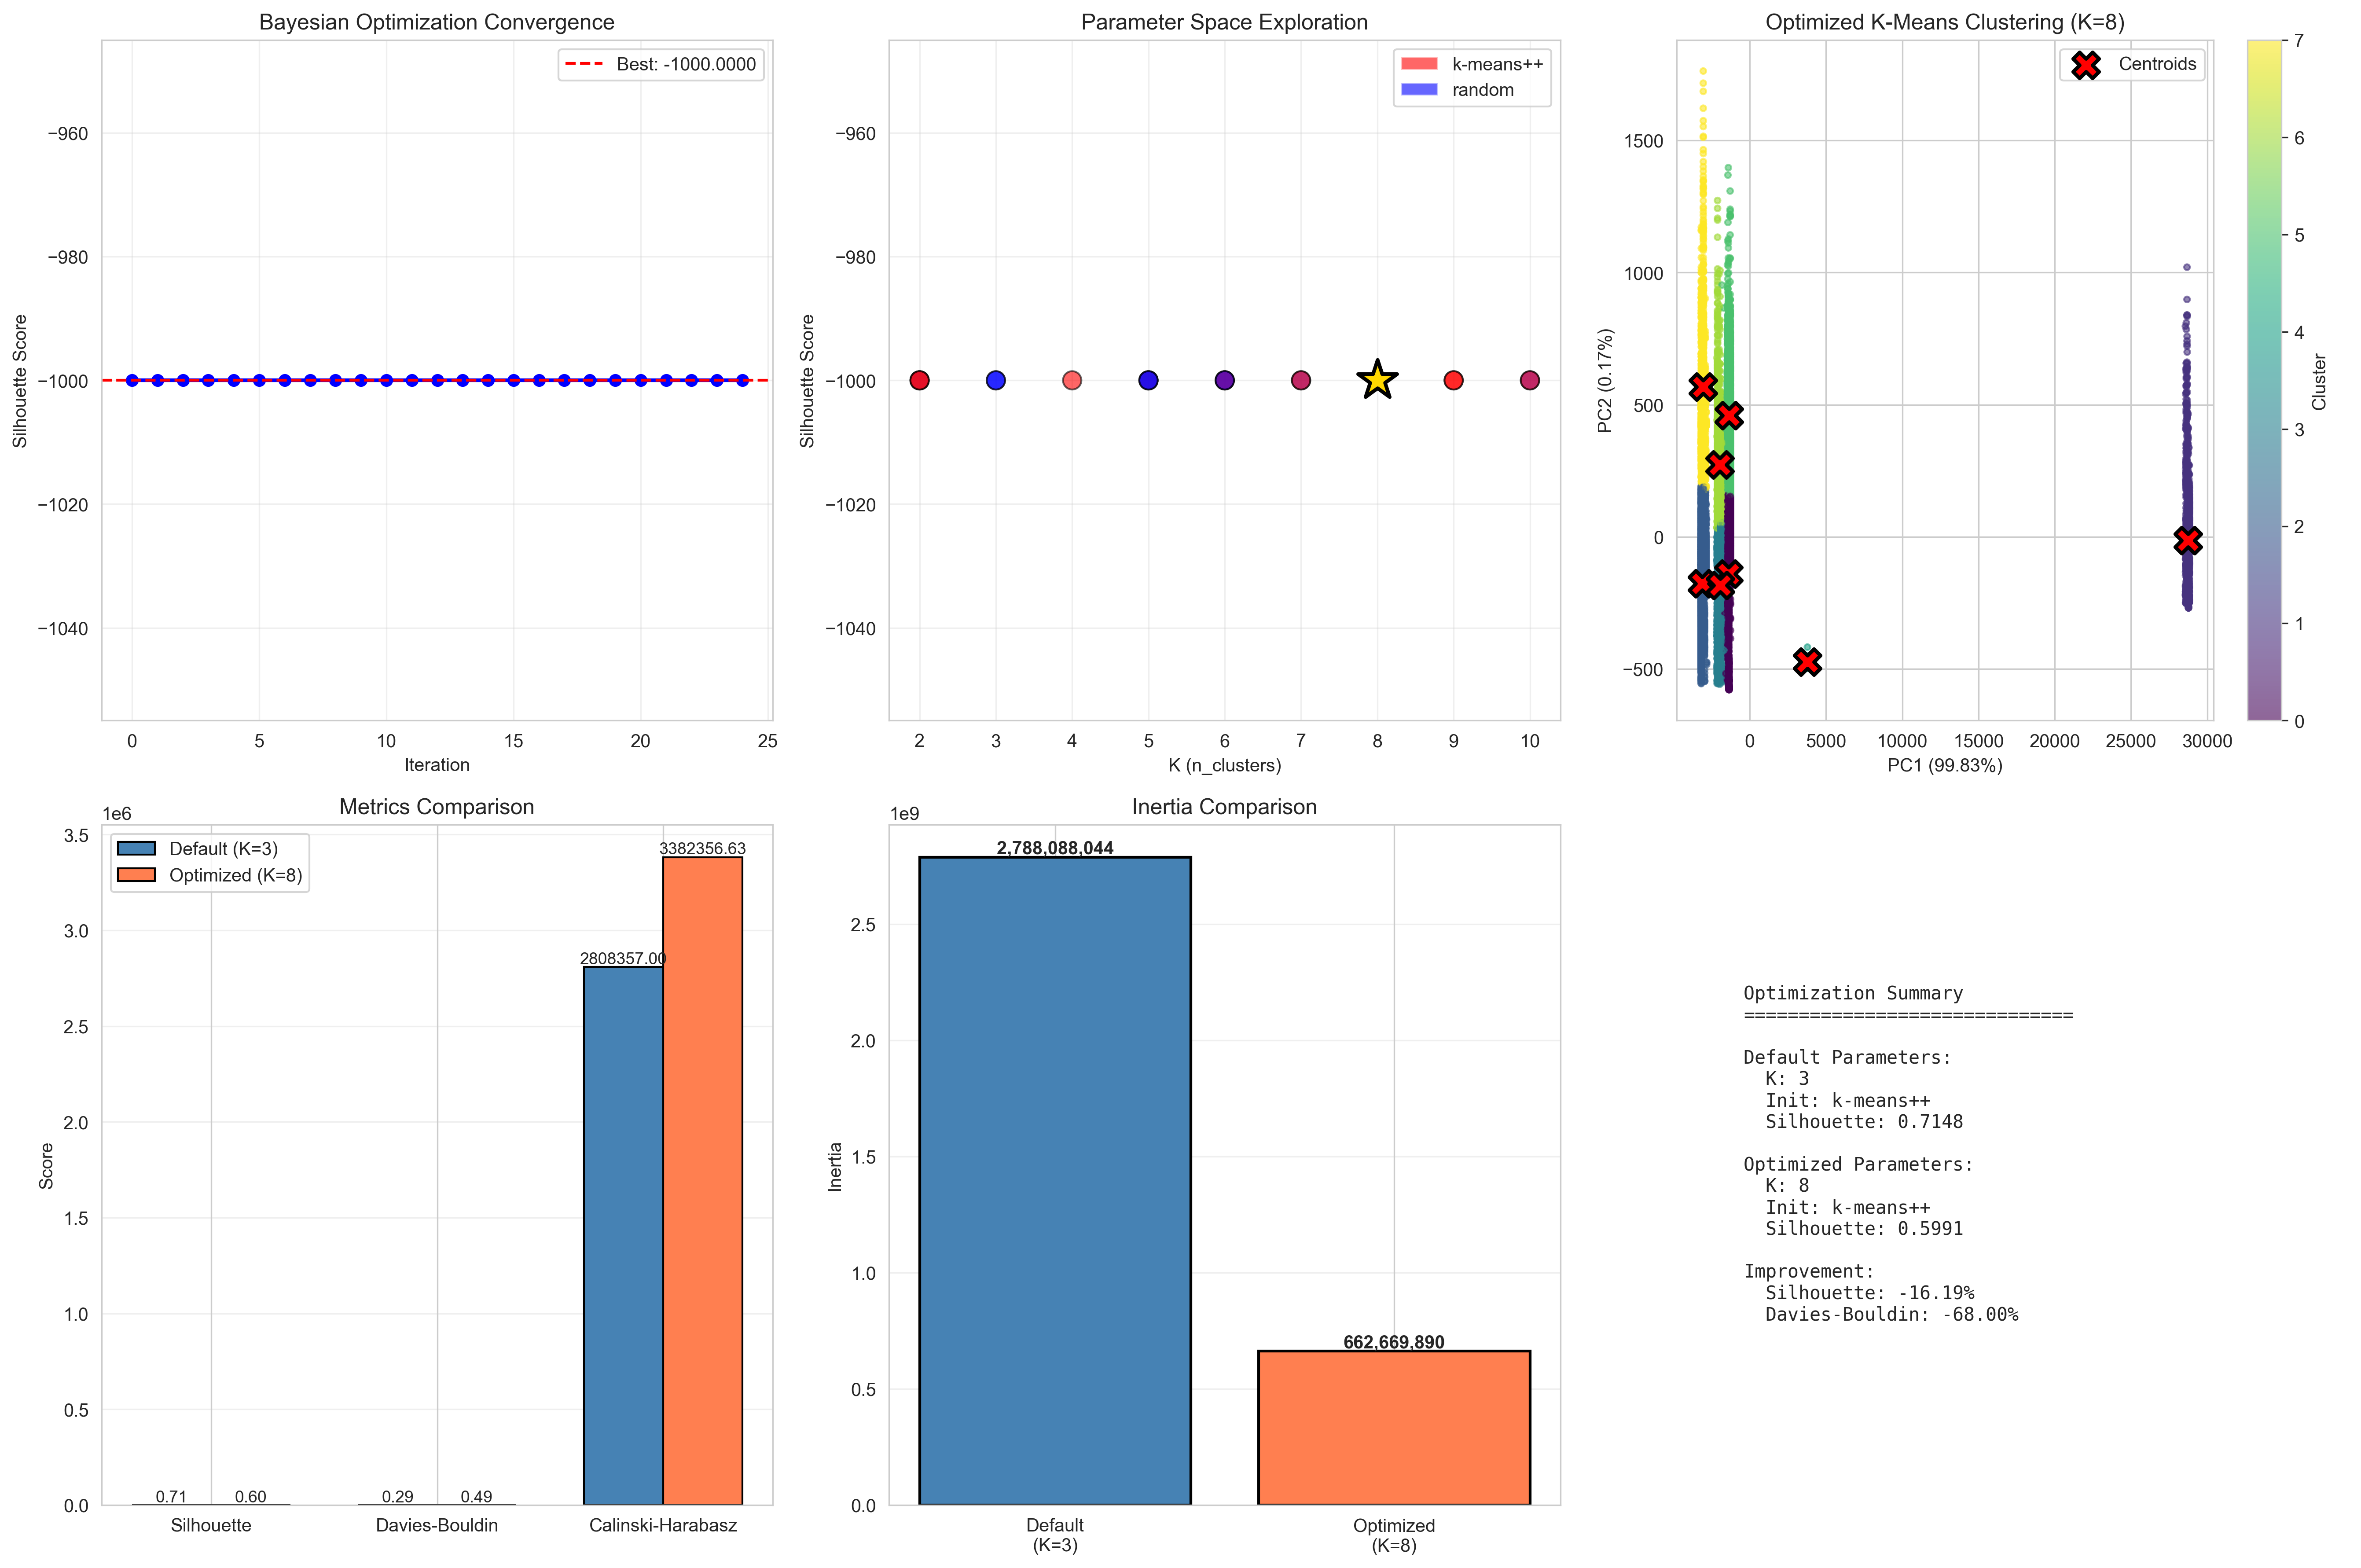
\includegraphics[width=0.8\linewidth]{images/Kmeans/kmeans_bayesian_optimization.png}
    \caption{Bayesian optimization applied to K-Means hyperparameters.}
    \label{fig:kmeans_bayesian_optimization}
\end{figure}
\subsection{From-Scratch K-Means Clustering ($K=5$)}

\paragraph{Cluster Visualization (PCA Projection)}
The PCA projection reveals one dominant cluster containing approximately $64\%$ of the samples, indicating a strong imbalance. Smaller clusters primarily capture outliers or edge cases rather than well-defined groups. Cluster centroids are mainly aligned along the first principal component, confirming the near one-dimensional structure of the data.

\paragraph{Cluster Size Distribution}
The cluster size distribution is highly imbalanced, suggesting that the clustering is driven by data density rather than underlying structure. This behavior indicates that the natural grouping of the data is closer to $2$ or $3$ clusters rather than $5$.

\paragraph{Silhouette Analysis}
The average Silhouette score is approximately $0.60$, reflecting acceptable but moderate clustering quality. The wide dispersion of silhouette values within clusters indicates internal inconsistency and partial overlap between clusters.

\paragraph{Performance Summary}
The algorithm achieves a reasonable runtime; however, the resulting clustering is more suitable for coarse segmentation than detailed profiling. The choice of $K=5$ already exceeds the structural capacity of the data.

\begin{figure}[H]
    \centering
    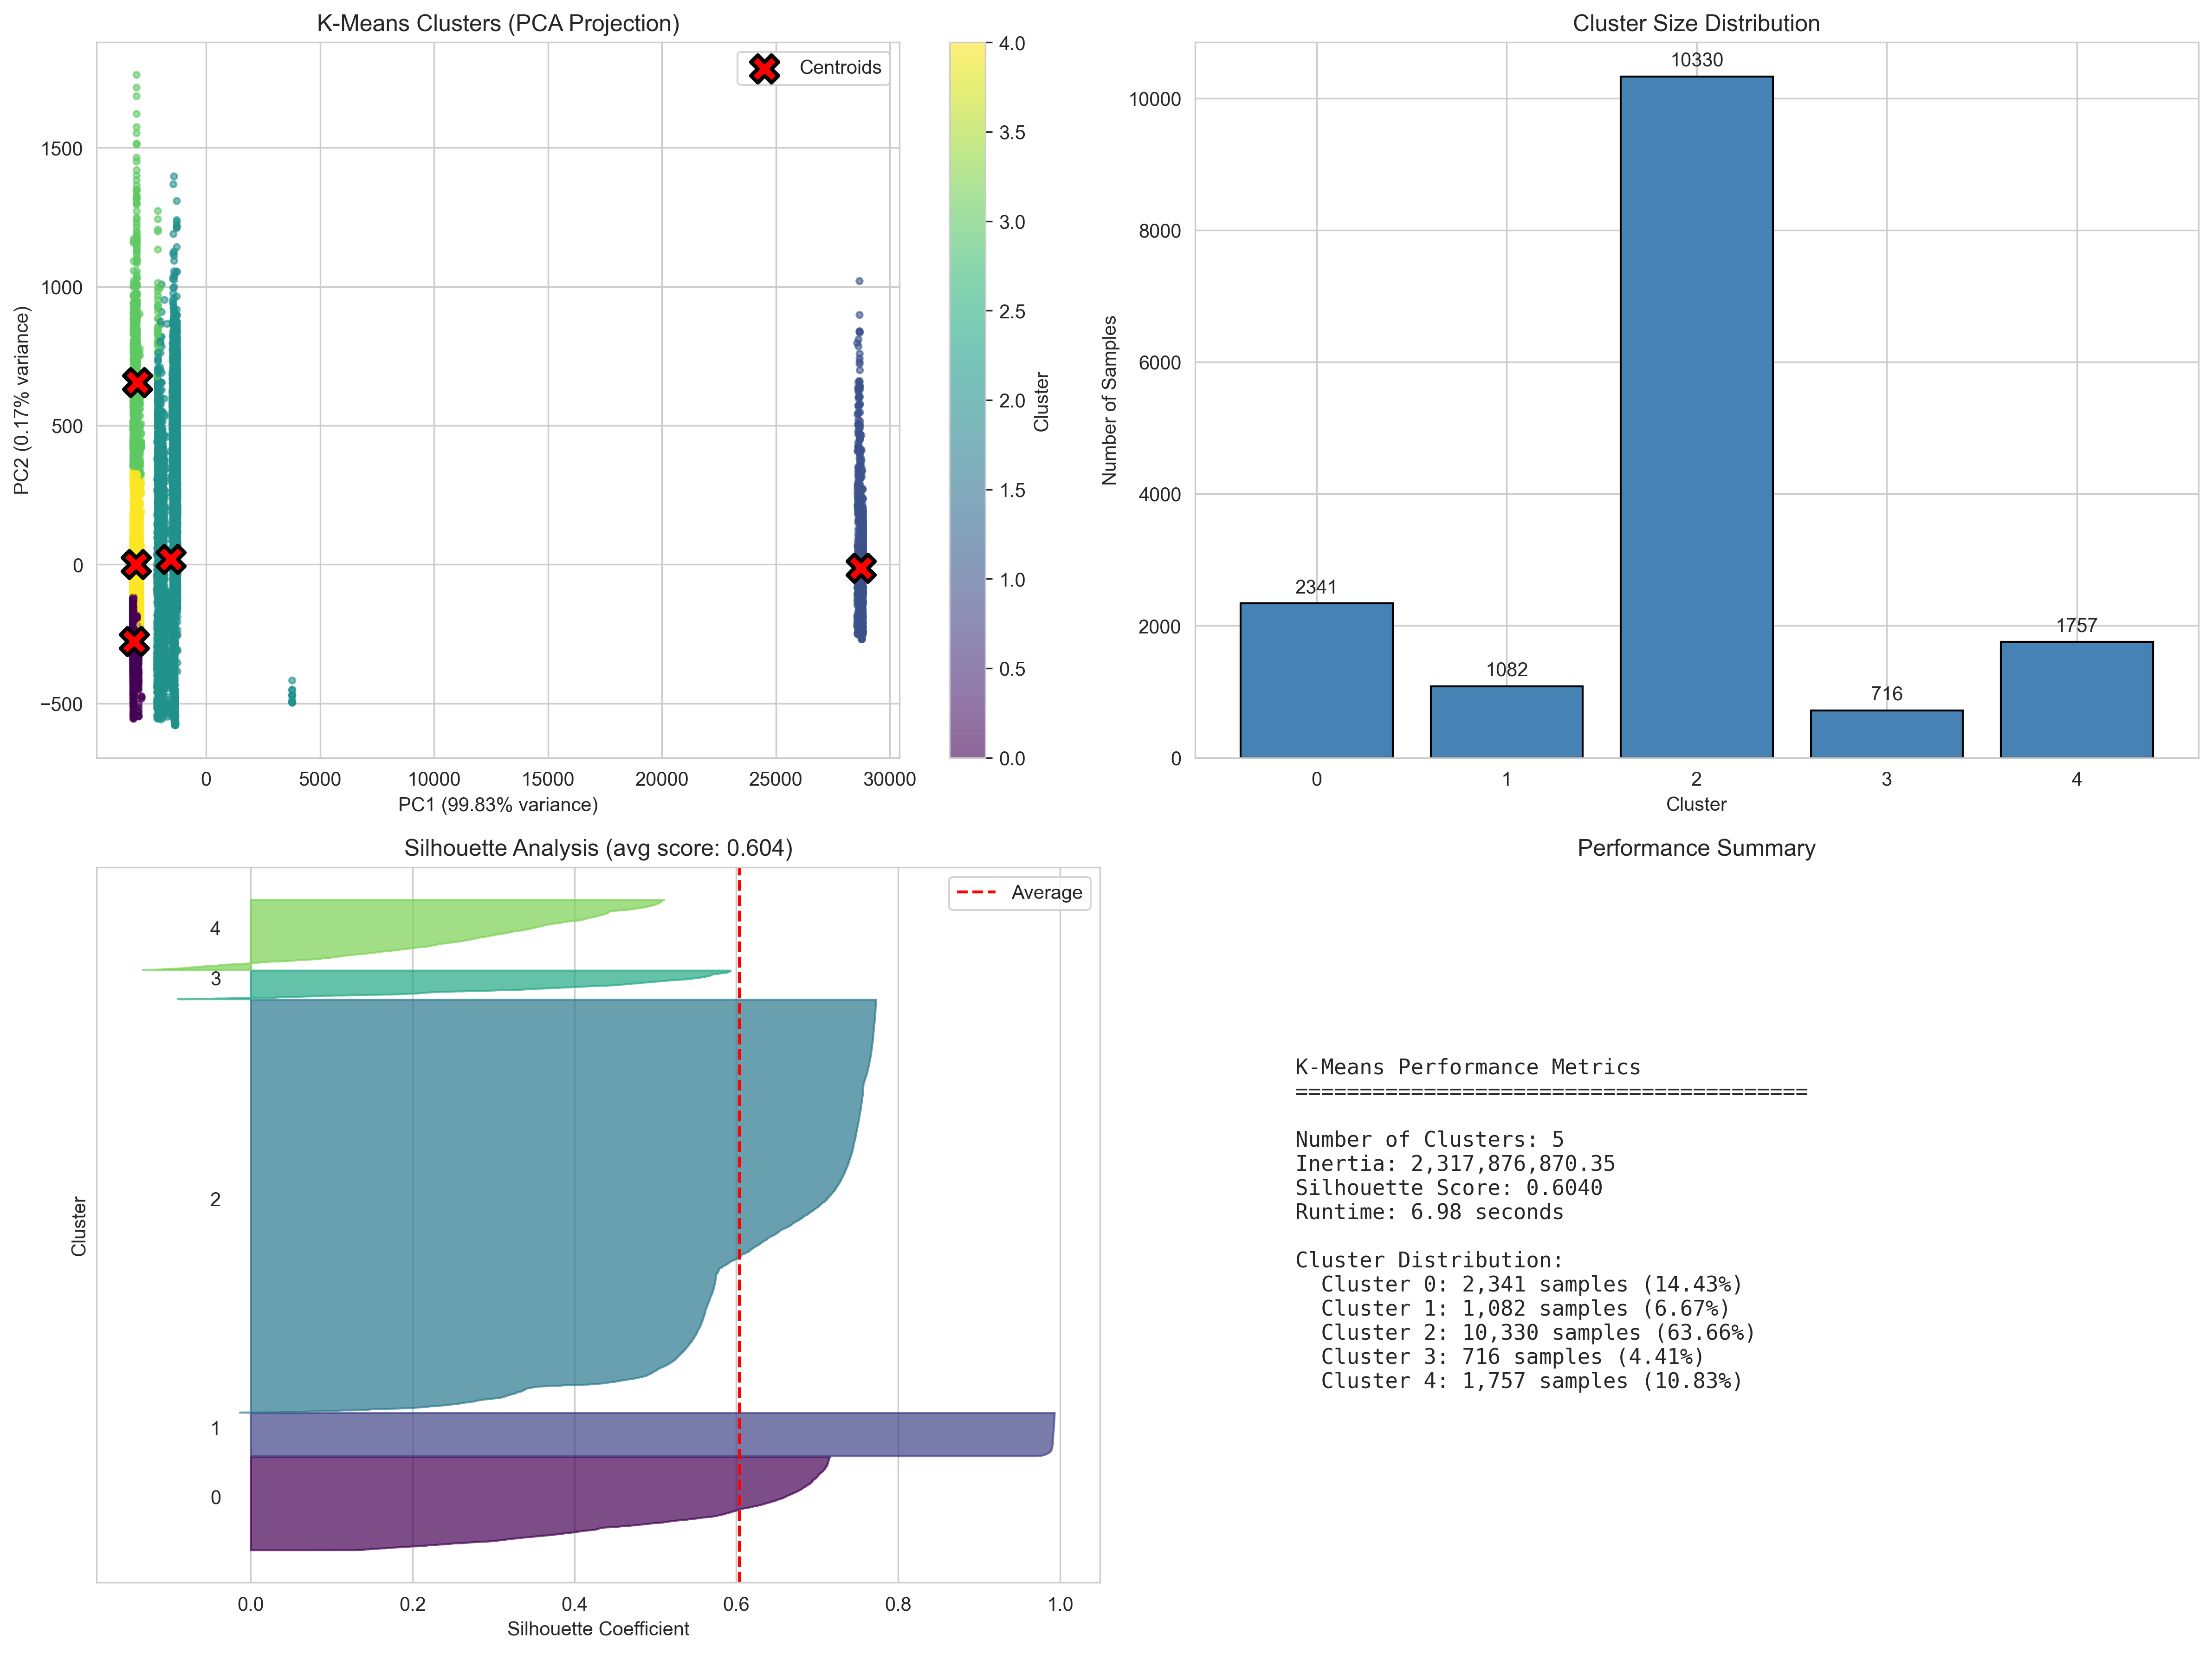
\includegraphics[width=0.8\linewidth]{images/Kmeans/kmeans_visualization_from_scratch.png}
    \caption{Visualization of K-Means clustering implemented from scratch.}
    \label{fig:kmeans_visualization_from_scratch}
\end{figure}

\subsection{Scikit-Learn K-Means Clustering ($K=3$)}

\paragraph{Cluster Visualization (PCA Projection)}
The PCA projection shows clear separation along the first principal component. Clusters are compact and well-defined, in agreement with the intrinsic low-dimensional structure of the data.

\paragraph{Cluster Size Distribution}
Although the cluster sizes remain imbalanced, the distribution is structurally meaningful. The dominant cluster reflects the true data density rather than overfitting or artificial fragmentation.

\paragraph{Silhouette Analysis}
The average Silhouette score is high (approximately $0.715$), with a narrow distribution of values, indicating strong internal cohesion and well-separated clusters. This configuration exhibits the best consistency between visual and quantitative evaluations.

\paragraph{Performance Summary}
The $K=3$ configuration provides the best balance between cluster separation, stability, and interpretability. The reduced number of clusters results in improved generalization.

\subsection{Overall Clustering Assessment}

The scikit-learn K-Means solution with $K=3$ is the most appropriate configuration for this dataset. Bayesian optimization did not yield meaningful improvements due to a flat objective surface and low metric sensitivity. Increasing the number of clusters mainly improves mechanical metrics such as inertia and the Calinski--Harabasz index, while degrading structural coherence. Given the effectively one-dimensional nature of the data, higher values of $K$ lead to unnecessary over-segmentation.

\begin{figure}[H]
    \centering
    
\includegraphics[width=0.8\linewidth]{images/Kmeans/sklearn_kmeans_visualization.png}
    \caption{Visualization of K-Means clustering using scikit-learn implementation.}
    \label{fig:sklearn_kmeans_visualization}
\end{figure}
